\documentclass[11pt,a4paper,fontset=windows]{ctexart}
\usepackage[margin=2.3cm]{geometry}
\usepackage{amsmath,amssymb}
\usepackage{graphicx}
\usepackage{booktabs}
\usepackage{multirow}
\usepackage{xcolor}
\usepackage[round,authoryear]{natbib}
\setcitestyle{aysep={,},yysep={,}}
\usepackage[colorlinks=true,linkcolor=blue!50!black,citecolor=blue!50!black,urlcolor=blue!50!black]{hyperref}
\urlstyle{same}
\usepackage{caption}
\captionsetup{font=small,labelfont=bf}
\graphicspath{{figures/}}
\DeclareMathOperator*{\argmin}{arg\,min}
\newcommand{\E}{\mathbb{E}}

\title{像人一样打 osu!：\\基于 TCN-WGAN 的光标轨迹生成与按键解码}
\author{pekin\\\small\url{https://github.com/pekingfather15/osuai}}
\date{2026 年 10 月}

\begin{document}
\maketitle

\begin{abstract}
本文从真人玩家的回放中训练神经网络，为节奏游戏 osu! 生成像人一样的游玩数据，并在 osu!lazer 中回放。
我们把这个任务表述为模仿学习：模型学习的是给定谱面时，玩家光标轨迹与按键的条件分布。
以 niooii 的开源项目为基础，我们收集了 1{,}992 份回放，在同一套评估标准下比较了四种成熟的深度学习序列模型
（LSTM、VAE、WGAN-GP 和时间卷积 WGAN）。最大的提升来自修正训练目标，而不是更换网络结构。我们证明了：
有限差分梯度惩罚只能测到判别器梯度的约 $1/\sqrt{d}=1/64$；平方误差损失必然把光标拉到转盘中心；
原评估使用的圆圈半径只有实际的一半。加入生成器预训练、转盘极坐标输出头、转盘统计损失并限制对抗权重后，
TCN-WGAN 在 46 张未见过的谱面上达到 99.89\% 的 Relax 准确率（真人 99.97\%），转盘转速 396 RPM（真人 371）。
在按键方面，我们发现游戏中损失的准确率大部分来自两个键几乎同时按下；把间隔小于 36\,ms（在验证集上选取）的按下合并后，
完整准确率从 93.55\% 提高到 95.45\%（真人 96.04\%）。在未登录状态下，系统在一张开启 Hidden 和 Hard Rock 的
7.11 星谱面上打出 96.63\%，按键时间的 UR 为 81。
\end{abstract}

\section{引言}
osu! 是一款节奏游戏：玩家把光标移到圆圈、滑条和转盘上，并踩着音乐的节拍按键。它也是 AI 主播 Neuro-sama 的起点：
在成为聊天型虚拟主播之前，Neuro-sama 是一个玩 osu! 的程序 \citep{neurosama}。本项目就是从这段经历开始的。

写一个完美打 osu! 的程序并不难，因为谱面文件写明了每个物件的位置和时间。更难、也更有意思的问题，
是让程序\emph{像人一样}打：光标轨迹平滑但不完美，会真正地转转盘，按键节奏自然。这也是本文所基于的
\citet{niooii} 项目的目标。这是一个机器学习问题：``像人''没有公式可写，只能从真人的游玩数据中学习。

本文的贡献：
\begin{itemize}
  \item 把任务表述为模仿学习中的条件生成建模，并据此解释 LSTM 这类确定性回归模型为什么学不会转盘；
  \item 基于 1{,}992 份回放的数据流程和固定的测试集 / 验证集划分，用谱面文件的哈希值排除测试谱面；
  \item 一套对生成数据和真人数据完全相同的评估方法，并用游戏内实测验证；
  \item 分析原 GAN 模型为何不会瞄准、不会转盘，给出修正，使 TCN-WGAN 成为最好的模型；
  \item 分析游戏中的按键失误，并提出能消除大部分失误的解码方法；
  \item 在目前开源的官方客户端 osu!lazer \citep{lazer} 中回放，且只允许在未登录状态下进行。
\end{itemize}

\section{背景}
\subsection{游戏机制}
一张谱面是一串物件，每个物件都有在 $512\times384$ 游戏区中的位置和出现时间。圆圈要准时点击；滑条要点击后按住键沿轨道跟随；
转盘要绕中心旋转。圆圈半径为 $r = 54.4-4.48\,\mathrm{CS}$ 个 osu! 像素，CS 为谱面的圆圈大小 \citep{wikics}。
判定窗口由整体难度 OD 决定：在物件时间前后 $80-6\,\mathrm{OD}$\,ms 内按下得 300，$140-8\,\mathrm{OD}$\,ms 内得 100，
$200-10\,\mathrm{OD}$\,ms 内得 50 \citep{wikiod}。OD 为 10 时，要拿 300 必须在 $\pm20$\,ms 内按下。准确率为
\begin{equation}
  \mathrm{acc}=\frac{300\,n_{300}+100\,n_{100}+50\,n_{50}}{300\,(n_{300}+n_{100}+n_{50}+n_{\mathrm{miss}})}.
  \label{eq:acc}
\end{equation}
玩家用 UR（unstable rate）衡量按键稳定度，即按键时间误差标准差（毫秒）的 10 倍。Relax 模组会自动按键，
因此在 Relax 下测得的准确率只反映光标的表现。

\subsection{人类的运动规律}
有两个经典结论描述了人的光标运动。Fitts 定律指出，到达目标所需的时间随 $\log_2(2D/W)$ 增长，
$D$ 为距离、$W$ 为目标宽度 \citep{fitts1954}，所以人在目标远或小时会放慢。最小加加速度（minimum-jerk）模型表明，
点到点的手臂运动会走最平滑的路径，即使加加速度（加速度的导数）平方的积分最小，从而产生平滑、钟形的速度曲线
\citep{flash1985}。人的运动还具有变化性：不同玩家、同一玩家的不同尝试，轨迹都不一样。
因此像人的模型既要生成平滑的轨迹，又要给出轨迹的\emph{分布}，而不是唯一答案。

\subsection{从示范中学习}
从专家的记录中学习行为称为模仿学习；最简单的形式是行为克隆，即把它当作从观测到动作的监督学习
\citep{pomerleau1989, hussein2017}。这里的观测是谱面 $x$（每个时间步的一组特征），动作是玩家的光标轨迹和按键状态 $y$。
行为克隆的一个已知弱点是协变量偏移：智能体自己的失误会把它带到专家从未到过的状态，误差不断累积 \citep{ross2011}。
我们的设定避开了这个问题，因为生成是开环的：整局在开始前就根据谱面全部生成好，游戏状态不会反馈给模型。

模型能学到什么，取决于用什么损失函数。用平方误差训练的模型学到的是条件均值：
\begin{equation}
  \argmin_f \E\left[\lVert y-f(x)\rVert^2\right] = \E[y \mid x]
  \label{eq:mean}
\end{equation}
\citep[第 1.5.5 节]{bishop2006}。当 $p(y\mid x)$ 只有一个峰时，均值是很好的答案，所以回归模型瞄得准；
当它有多个峰时，均值可能是没有任何人会给出的答案。在转盘上，玩家绕中心画的圆相位各不相同；
对相位 $\phi$ 取平均，$\E_\phi[c + r(\cos\phi,\sin\phi)] = c$，恰好是中心本身。因此确定性回归模型在转盘上会一动不动。
要像人，模型必须从 $p(y\mid x)$ 中\emph{采样}，而这就是生成模型的用途。

\section{模型}
本文所有模型都是用梯度下降训练的深度神经网络。第~\ref{sec:frontier} 节把它们与当前的前沿模型作比较。

\subsection{循环神经网络与 LSTM}
循环神经网络逐步读取序列，用隐藏状态 $h_t$ 概括过去的信息。普通循环网络很难在长序列上训练，因为梯度在多步反向传播中会消失或爆炸。
长短期记忆网络（LSTM）增加了一个以加法更新、由门控制的细胞状态 $c_t$ \citep{hochreiter1997, gers2000}：
\begin{align}
  i_t,\,f_t,\,o_t &= \sigma\left(W\,[h_{t-1},x_t] + b\right), \qquad
  \tilde c_t = \tanh\left(W_c\,[h_{t-1},x_t] + b_c\right),\\
  c_t &= f_t\odot c_{t-1} + i_t\odot \tilde c_t, \qquad h_t = o_t\odot\tanh(c_t),
\end{align}
其中输入门、遗忘门、输出门 $i_t, f_t, o_t$ 分别决定写入、保留和读出什么。LSTM 曾被用来从笔迹轨迹生成人的手写
\citep{graves2013}，与本文的任务很接近。但用平方误差（或本文实际使用、在小误差时同样是平方形式的 Huber 损失）训练时，LSTM 是一个回归模型，输出的是式~\eqref{eq:mean} 中的平均轨迹。

\subsection{时间卷积网络}
时间卷积网络（TCN）用堆叠的一维卷积代替循环。因果卷积只使用 $t$ 时刻及之前的输入；卷积核大小为 $k$、空洞率为 $d$ 的空洞卷积
读取 $t, t-d, \dots, t-(k-1)d$ 处的输入 \citep{yu2016, oord2016}。每层空洞率翻倍，感受野就随深度指数增长：
\begin{equation}
  R = 1 + (k-1)\sum_{\ell=1}^{L} d_\ell, \qquad d_\ell = 2^{\ell-1}.
\end{equation}
TCN 可以并行处理所有时间步，在许多序列任务上与 LSTM 相当甚至更好，并且有效记忆更长 \citep{bai2018}。
由于整张谱面事先已知，我们还可以让部分层向未来偏移。卷积还支持梯度惩罚所需的二阶导数，而 cuDNN 中的 LSTM 不支持（见 5.1 节）。

\subsection{变分自编码器}
变分自编码器（VAE）学习一个带先验 $p(z)$ 的隐变量模型 $p_\theta(y\mid z,x)$。由于似然无法直接计算，
用编码器 $q_\phi(z\mid y,x)$ 近似后验，二者共同最大化证据下界 \citep{kingma2014vae, rezende2014}：
\begin{equation}
  \log p_\theta(y\mid x) \ge \E_{q_\phi(z\mid y,x)}\left[\log p_\theta(y\mid z,x)\right]
  - \mathrm{KL}\left(q_\phi(z\mid y,x)\,\Vert\,p(z)\right).
\end{equation}
对 $z$ 采样，同一张谱面就能得到不同的输出。但当解码器足够强时，模型可以忽略 $z$，把 KL 项压到零；
这种\emph{后验坍塌} \citep{bowman2016} 会让 VAE 退化为均值预测器。对抗式 VAE 加入判别器来提高真实感 \citep{plumerault2020}。

\subsection{生成对抗网络与 WGAN-GP}
生成对抗网络（GAN）让生成器 $G(z,x)$ 与判别器对抗训练，判别器试图分辨真实数据和生成数据 \citep{goodfellow2014}；
两者都以 $x$ 为条件时就是条件 GAN \citep{mirza2014}。原始目标训练不稳定，容易出现模式坍塌，即生成器只覆盖少数几个峰。
Wasserstein GAN 改为最小化推土机距离，由 Kantorovich--Rubinstein 对偶性，
\begin{equation}
  W(p_r,p_g)=\sup_{\lVert D\rVert_L\le 1}\;\E_{y\sim p_r}[D(y)]-\E_{y\sim p_g}[D(y)],
\end{equation}
其中判别器 $D$ 必须满足 1-Lipschitz 条件 \citep{arjovsky2017}。WGAN-GP 在真实样本与生成样本之间的随机插值点 $\hat y$
上施加梯度惩罚来实现这一约束 \citep{gulrajani2017}：
\begin{equation}
  \mathcal{L}_{\mathrm{GP}} = \lambda\,\E_{\hat y}\left[\left(\lVert\nabla_{\hat y} D(\hat y)\rVert_2-1\right)^2\right].
  \label{eq:gp}
\end{equation}
计算 $\nabla_\theta\mathcal{L}_{\mathrm{GP}}$ 需要对梯度再求导（二阶反向传播）。对抗损失常与让输出贴近目标的重建损失结合使用，
例如图像到图像的转换 \citep{isola2017}；本文也是如此。

\subsection{与前沿的关系}
\label{sec:frontier}
这些结构都不新：LSTM 提出于 1997 年，VAE 和 GAN 于 2014 年，WGAN-GP 于 2017 年，本文所用的 TCN 评估于 2018 年。
它们是成熟的方法，选用它们是因为适合 10{,}730 段训练数据和一块笔记本显卡的规模，也因为原项目实现了它们。
序列与动作生成的前沿已经转向 Transformer \citep{vaswani2017}、去噪扩散模型 \citep{ho2020}
（已能以很高的真实感生成人体动作 \citep{tevet2023}）以及 Mamba 等状态空间模型 \citep{gu2023}。这些模型更大，也更依赖数据。
本文没有提出新的结构，而是分析成熟方法在这个任务上为何失败，再根据上述原理加以修正。

\subsection{osu! 相关工作}
OsuLearn 用循环网络从回放学习生成光标运动 \citep{osulearn}。\citet{niooii} 在此基础上加入了 VAE、以 LSTM 为判别器的 WGAN-GP
和 TCN-WGAN，并在视频中给出一张谱面上的 Relax 准确率：LSTM 98.10\%、VAE 98.89\%、LSTM-WGAN 99.68\%、TCN-WGAN 99.40\%。
作者提到 LSTM 打得``太好''、很机械，VAE 会把动作平均化、不能稳定地学会转盘，TCN 版本``可能没有调好''。
按键由另一个 LSTM 生成，作者称它``在较难的段落有时会按两下''。本文发现，这种重复按键是游戏中掉分的主要原因。
其他开源项目有为谱面编辑器生成光标运动的 \citep{osucad}，也有基于截屏和目标检测来打图的 \citep{autosu}。

\section{数据}
\paragraph{来源。} 从官网下载了世界排名第一和第三的两位玩家的回放（671 份）。为了覆盖更多玩家，又导入了 osu!3k 数据集
\citep{osu3k}（MIT 许可）：按玩家 pp 从高到低选取准确率 $\ge 90\%$、星级 $\ge 5$ 的回放，排除会改变玩法的模组
（Relax、Autopilot、Spun Out、Easy、Half Time）。谱面从镜像站下载，并按谱面文件的 MD5 与回放匹配。

\paragraph{清洗。} osu!3k 中有些条目是同一份操作以不同模组重复渲染的，这类相互矛盾的重复全部丢弃。
另有 20 份回放来自总 pp 不足 2{,}000、却打出高星高准成绩的玩家，判定为可疑并排除。

\paragraph{划分。} 测试集 50 份回放（有效 46 份），均在 V1 训练之后下载，谱面从未用于训练，每张谱面一份。
验证集 30 份（有效 27 份），只用于挑选存档和解码参数。从 V3 起按文件哈希值（而非路径）排除测试和验证谱面，
额外拦下了 9 份存放在其他文件夹、实为同一谱面的回放。

\paragraph{表示。} 每张谱面转换为 12\,ms 一帧的序列，每帧 9 个特征：下一个物件的位置、距它的时间、物件类型、CS、
滑条速度和长度。目标是光标位置和两个按键的状态。序列切成 2{,}048 帧（24.6\,s）一段。

\begin{table}[t]
\centering
\caption{数据集版本。一段为 2{,}048 帧，每帧 12\,ms。}
\label{tab:data}
\begin{tabular}{lll}
\toprule
版本 & 训练回放 & 段数 \\
\midrule
V1 & 212 份（两位玩家） & 1{,}409 \\
V2 & 425 份（两位玩家） & 2{,}530 \\
V3 & 1{,}992 份（官网 671 + osu!3k 1{,}410；1{,}000 多名玩家） & 10{,}730 \\
\midrule
\citet{niooii} & -- & 13{,}617 \\
\bottomrule
\end{tabular}
\end{table}

\section{方法}
\subsection{TCN-WGAN 光标模型}
生成器是卷积核为 3 的 TCN，输入为谱面特征拼接 8 维噪声序列。前六层（空洞率 1 到 32）每层把卷积核向未来移两帧，
因此生成器能看到 12 帧（144\,ms）之后的内容；后四层为因果卷积，总共能看到 1.7\,s 的过去。判别器是以谱面特征和一段光标轨迹为输入的 TCN，
七个空洞层每层向未来看一帧，对整段输出一个分数。生成器 277{,}956 个参数，判别器 141{,}025 个。生成器的损失为
\begin{equation}
  \mathcal{L}_G = \mathcal{L}_{\mathrm{pos}} - \lambda_{\mathrm{adv}}\,\E[D(G(z,x),x)] + \lambda_{\mathrm{spin}}\,\mathcal{L}_{\mathrm{spin}},
\end{equation}
其中 $\mathcal{L}_{\mathrm{pos}}$ 为位置的 Huber（smooth L1）误差：误差小于 1 时它是平方形式，所以瞄准时的表现与式~\eqref{eq:mean} 的平方误差相同。判别器使用式~\eqref{eq:gp} 的标准惩罚，$\lambda=8$，每步生成器训练对应三步判别器训练。
优化器为 Adam \citep{kingma2015}，$\beta=(0.5,0.9)$。

\paragraph{原梯度惩罚为何失效。} 原 WGAN 代码为了避免在 LSTM 判别器上做二阶反向传播，把式~\eqref{eq:gp} 换成了沿一个随机单位方向 $u$
的有限差分：$(D(\hat y+\epsilon u)-D(\hat y))/\epsilon \approx u^\top g$，其中 $g=\nabla D(\hat y)$。当 $u$ 在 $\mathbb{R}^d$
的单位球面上均匀分布时，$\E[(u^\top g)^2]=\lVert g\rVert^2/d$，所以 $|u^\top g|\approx\lVert g\rVert/\sqrt d$。
一段 2{,}048 帧、每帧 $(x,y)$ 的轨迹有 $d=4{,}096$ 维，惩罚项只看到梯度的 $1/64$，于是把 $\lVert g\rVert$ 推向 64 而不是 1。
判别器因此远离 1-Lipschitz；实验中其损失停在 3.66 左右，Wasserstein 距离估计始终接近 0，说明它无法区分真实与生成的游玩。
在 LSTM 判别器上使用标准惩罚每步需要 12.2\,s（cuDNN 的 LSTM 不支持二阶求导），而近似版只需 0.13\,s，不可行；
卷积判别器则能低成本地计算标准惩罚，这就是我们选用 TCN 的原因。

\paragraph{预训练。} 原学习率 $10^{-4}$ 训练 100 轮后位置误差仍在下降。我们先只用 $\mathcal{L}_{\mathrm{pos}}$ 以 $10^{-3}$ 训练生成器 60 轮，
再以 $10^{-4}$ 进行对抗训练，$\lambda_{\mathrm{adv}}$ 逐渐增大，上限为 $2\times10^{-4}$。更大的权重会让判别器分数膨胀，把光标拉离目标。

\paragraph{转盘。} 根据式~\eqref{eq:mean}，转盘帧上的位置损失会把光标拉向中心，因此我们把转盘帧从 $\mathcal{L}_{\mathrm{pos}}$ 中去掉。
另设一个极坐标输出头，在转盘期间输出半径 $r_t$ 和角速度 $\omega_t$：
\begin{equation}
  (x_t,y_t)=c+r_t\,(\cos\theta_t,\sin\theta_t),\qquad \theta_t=\theta_0+s\sum_{\tau\le t}\omega_\tau,
\end{equation}
其中 $c$ 为游戏区中心，起始角度 $\theta_0$ 和方向 $s\in\{-1,1\}$ 由噪声决定。独立的输出头使转盘训练不会干扰瞄准。
转盘统计损失只要求平均角速度 $\bar\omega$ 不低于真人、平均半径 $\bar r$ 与真人相近，而不要求特定相位，所以不存在平均化问题：
\begin{equation}
  \mathcal{L}_{\mathrm{spin}}=\max(0,\bar\omega_{\mathrm{real}}-\bar\omega_{\mathrm{fake}})
  +\left(\frac{\bar r_{\mathrm{fake}}-\bar r_{\mathrm{real}}}{100}\right)^2,
\end{equation}
$\lambda_{\mathrm{spin}}=0.02$，从第 30 轮开始启用。

\subsection{按键模型与解码}
按键沿用原作者的按键模型：两层 LSTM（64 维）加全连接层，逐帧预测两个键各自处于按住状态的概率（54{,}626 个参数），
以真人按键状态为目标、用二元交叉熵训练。这种表述方式有两个性质导致了失误。第一，按下只占一帧，按住却持续五到十帧，
损失由按住帧主导，按下时刻差一帧时损失几乎不变；按下事件很稀少，这是目标检测中常见的类别不平衡问题 \citep{lin2017}。
第二，模型经常拿不准真人会用哪个键，两个概率都在 0.5 附近徘徊，对每个键单独设阈值就会在一两帧内把两个键都按下
（图~\ref{fig:keys}）。在游戏中，每次多出的按键都可能提前打到下一个物件；而 osu!lazer 中只有打中滑条头的那个键能维持滑条跟随，
所以一次先到达滑条头、随即松开的短按会让滑条尾丢失。

为此我们对按键进行解码：开始时间相隔小于 $g$ 的按下合并为一次，按住到其中最晚松开的时刻；再给每次按下分配一个当前没有按住的键，
同一个键要先松开一帧才能再按。目标检测中的非极大值抑制也是这样合并近乎重复的检测结果的 \citep{neubeck2006}。间隔 $g$ 在验证集上选取。

\begin{figure}[t]
\centering
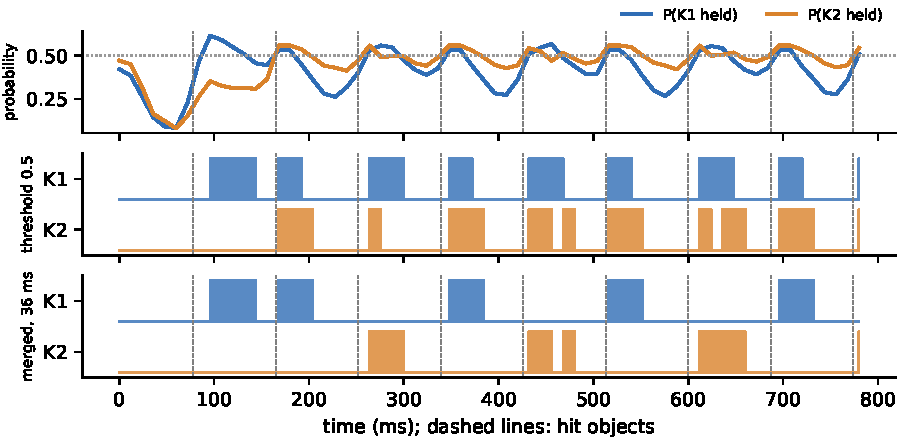
\includegraphics[width=\linewidth]{key_decoding.pdf}
\caption{7.88 星谱面上一段 800\,ms 连打中的按键模型输出。上：按住概率。中：每个键单独以 0.5 为阈值，几乎每个物件都两个键一起按。
下：合并间隔小于 36\,ms 的按下之后。按键也略晚于物件（全图平均晚 7\,ms），由回放的 offset 补偿。}
\label{fig:keys}
\end{figure}

\subsection{在 osu!lazer 中回放}
原回放程序读取 osu!stable 的内存。对于 osu!lazer，我们从 tosu \citep{tosu} 的 websocket 读取游戏状态：谱面文件、歌曲时间、模组和账号信息。
歌曲时间每 10--20\,ms 更新一次，两次更新之间用本地时钟推算，并且不允许小于 50\,ms 的回退。光标按 lazer 的游戏区变换
（缩放 $h/480$，居中）换算到屏幕坐标。跳过的帧中的按键变化按顺序补发，另用 offset 补偿回放延迟。一个小窗口程序在选中谱面时生成游玩，也可以只生成光标、配合 Relax 模组测试；只有当 tosu 报告未登录时才允许回放。

\subsection{代码实现}
V3 模型是用本项目的第一版代码训练的，第一版建立在 \citet{niooii} 的代码之上。之后，仓库里的所有代码都为本项目重新编写：
谱面与回放解析（滑条曲线改为按 .osu 格式的曲线类型计算，不再使用粗略近似）、特征、模型、训练、评估和回放。
V3 的权重已转换到新代码，同样的输入得到完全相同的输出。第 7.1 和 7.2 节的结果来自第一版代码；按键解码的结果和表~\ref{tab:keys} 用新代码重新计算。

\section{评估方法}
对测试集中的每份回放，模型为同一张谱面、同样的模组生成一局，生成数据和真人数据用同一套标准评分：
\begin{itemize}
  \item \textbf{Relax 准确率}：对每个圆圈或滑条头，在其 50 判定窗口内找光标位于圆圈内、且离物件时间最近的时刻来判定，相当于由游戏代为按键。
  \item \textbf{完整准确率}：结合按键判定。两个键的每次按下只能打一个物件；物件取其判定窗口内最早一次、且光标在圆圈内的未用按键。
  \item \textbf{滑条尾}：打中滑条头的那个键必须一直按住，光标也须留在跟随圈（$2.4r$）内，直到滑条结束前 36\,ms。
  \item \textbf{转盘转速}：转盘期间绕游戏区中心的转速。
\end{itemize}
原评估代码使用的圆圈半径只有实际的一半；除特别说明外，本文数字均使用修正后的半径。完整准确率会低估实际准确率：
真人回放在此标准下为 95.84\%，而回放文件记录的是 99.00\%，主要因为 12\,ms 采样会丢掉部分短促的按键。尽管如此，
该评估能可靠地预测实战：对下文 7.88 星的谱面，它预测 90.63\%、滑条尾 391/420，游戏实测为 90.09\%、393/420。
重写后的评估复现了第一版的结果：在同样的 46 局测试回放上，V3 TCN-WGAN 不合并按键时完整准确率为 93.44\%，合并后为 95.47\%
（第一版为 93.41\% 和 95.49\%），Relax 准确率（99.89\%）、命中率、平均偏差和转盘转速完全相同。
新的解析器还能读取第一版读不了的 4 张测试谱面，所以下文的表格使用全部 50 局。

\section{实验结果}
\subsection{光标模型}
表~\ref{tab:main} 在 46 张测试谱面上比较了所有模型（按键模型相同），图~\ref{fig:traj} 展示了它们的轨迹。

\begin{table}[t]
\centering
\caption{测试集（46 张未见过的谱面），第一版代码，修正半径，均搭配 V3 按键模型（不合并按键，完整准确率为第一版判定）。}
\label{tab:main}
\small
\begin{tabular}{lrrrrr}
\toprule
来源 & 完整准确率 & Relax 准确率 & Relax Miss & 平均偏差 & 转盘 \\
\midrule
真人 & 95.84\% & 99.97\% & 5 & 11.9\,px & 371 RPM \\
V1 LSTM & 94.94\% & 99.95\% & 14 & 9.1\,px & 3 \\
V1 WGAN-GP & 62.53\% & 80.49\% & 4{,}988 & 33.7\,px & 41 \\
V2 LSTM & 94.79\% & 99.96\% & 13 & 9.7\,px & 6 \\
V2 VAE & 51.92\% & 71.13\% & 8{,}219 & 39.1\,px & 42 \\
V2 WGAN-GP & 81.55\% & 91.95\% & 2{,}482 & 24.3\,px & 34 \\
V2 TCN-WGAN（原作者设置） & 73.19\% & 91.17\% & 1{,}962 & 26.3\,px & 29 \\
V3 LSTM & 94.76\% & 99.92\% & 27 & 10.6\,px & 3 \\
\textbf{V3 TCN-WGAN} & \textbf{94.68\%} & \textbf{99.89\%} & \textbf{28} & \textbf{8.3\,px} & \textbf{396} \\
\bottomrule
\end{tabular}
\end{table}

\begin{figure}[t]
\centering
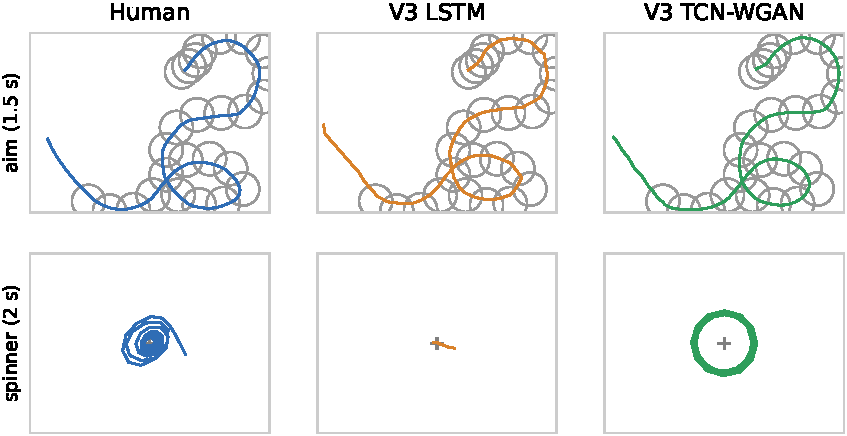
\includegraphics[width=0.92\linewidth]{trajectories.pdf}
\caption{一张未见过的谱面上的光标轨迹。上：1.5\,s 的瞄准段。下：转盘的前 2\,s。LSTM 瞄得和 GAN 一样准，
但正如式~\eqref{eq:mean} 所预测的，它停在转盘中心。}
\label{fig:traj}
\end{figure}

结果与第 2 节的原理一致。LSTM 几乎完美地瞄准，这符合回归模型在单峰目标上的预期，但它从不转盘（3--6 RPM）。
VAE 的 KL 项在所有版本中都趋于零，即发生了后验坍塌，使它仍是均值预测器；而且它的转盘损失也是位置损失。
原作者的 GAN 模型瞄准较差，我们把原因追溯到梯度惩罚和学习率。修正之后，V3 TCN-WGAN 瞄得和 LSTM 一样准，转盘也像真人。
更多样的数据（V3，上千名玩家）让 LSTM 略有下降，因为它的平均轨迹混合了更多风格；却让 GAN 受益，因为 GAN 能从风格的分布中采样。

\subsection{消融实验}
表~\ref{tab:ablation} 在 V2 数据上逐项加入修正。这些数字使用旧的（减半的）半径，只适合相互比较。

\begin{table}[t]
\centering
\caption{TCN-WGAN 在 V2 数据上的消融实验（测试集，旧的减半半径）。}
\label{tab:ablation}
\begin{tabular}{lrrr}
\toprule
改动 & Relax 准确率 & 平均偏差 & 转盘 \\
\midrule
原作者设置（100 轮，学习率 $10^{-4}$） & 56.5\% & 26.6\,px & 24 RPM \\
+ 生成器预训练（40 轮，学习率 $10^{-3}$） & 96.7\% & 10.1\,px & 26 \\
+ 转盘帧不计位置损失、加转盘统计损失（共享输出） & 89.9\% & 14.7\,px & 86 \\
+ 转盘极坐标输出头 & 89.3\% & 14.5\,px & 372 \\
+ 预训练 60 轮，$\lambda_{\mathrm{adv}}\le 2\times10^{-4}$ & 97.4\% & 9.5\,px & 519 \\
\bottomrule
\end{tabular}
\end{table}

\begin{figure}[t]
\centering
\begin{minipage}{0.48\linewidth}
\centering
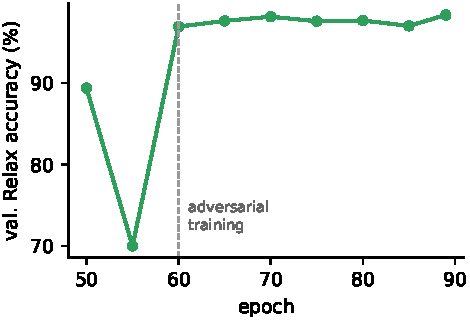
\includegraphics[width=\linewidth]{checkpoints.pdf}
\caption{V3 TCN-WGAN 各存档在验证集上的表现（旧半径），选用第 89 轮。}
\label{fig:ckpt}
\end{minipage}\hfill
\begin{minipage}{0.48\linewidth}
\centering
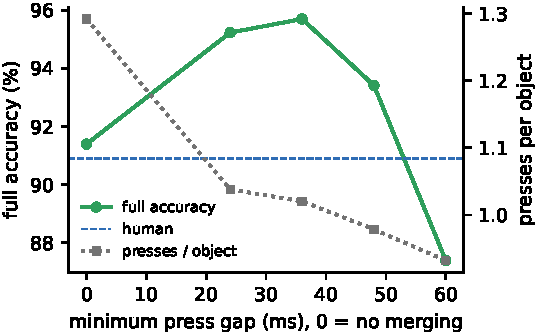
\includegraphics[width=\linewidth]{gap_sweep.pdf}
\caption{在验证集上选取按键合并间隔。}
\label{fig:gap}
\end{minipage}
\end{figure}

仅预训练一项就把 Relax 准确率从 56.5\% 提高到 96.7\%。瞄准与转盘共享输出会损失准确率，独立的极坐标输出头和更低的对抗权重把它找了回来。
各存档之间的准确率波动很大（第 55 轮 70\%，第 60 轮 97\%；图~\ref{fig:ckpt}），这在对抗训练中很常见，因此必须用验证集挑选存档。

\subsection{按键解码}
判定已更新为分别统计两个键的按下，并计入滑条尾。图~\ref{fig:gap} 和表~\ref{tab:keys} 显示，合并间隔小于 36\,ms 的按下后，
每个物件的按键次数从 1.29 降到 1.02（真人 1.00），验证集上的完整准确率超过了真人回放。间隔再大，就会开始合并快速连打中真实的按键。

\begin{table}[t]
\centering
\caption{按键解码，V3 TCN-WGAN 搭配 V3 按键模型，用重写后的评估计算（验证集 30 局，测试集 50 局）。}
\label{tab:keys}
\small
\begin{tabular}{llrrrr}
\toprule
数据集 & 解码 & 完整准确率 & 300/100/50/Miss & 滑条尾 & 每物件按键 \\
\midrule
\multirow{4}{*}{验证集} & 真人 & 90.89\% & 20906/1482/31/1131 & 94.3\% & 1.00 \\
 & 阈值 0.5 & 91.39\% & 20856/1555/890/249 & 94.5\% & 1.29 \\
 & 合并 24\,ms & 95.23\% & 22097/881/215/357 & 96.4\% & 1.04 \\
 & 合并 36\,ms & 95.70\% & 22270/739/124/417 & 96.4\% & 1.02 \\
\midrule
\multirow{3}{*}{测试集} & 真人 & 96.04\% & 37150/2244/31/40 & 99.4\% & 1.03 \\
 & 阈值 0.5 & 93.55\% & 36052/2108/982/323 & 95.3\% & 1.16 \\
 & \textbf{合并 36\,ms} & \textbf{95.45\%} & 37259/1031/405/770 & 95.8\% & 1.00 \\
\bottomrule
\end{tabular}
\end{table}

合并消除了大部分 50，但 Miss 增加了（测试集从 323 到 770）：有些真实的按键也被合并掉了。
用同样方法评估的 V3 LSTM 合并后为 95.74\%：它的按键来自同一个按键模型，瞄得也略准一些，但它不会转盘（3 RPM）。
模型学的是按住状态而不是按下事件，单靠解码无法彻底解决。

\section{游戏内实测}
所有实测均在 osu!lazer 中以未登录（游客）状态进行，全屏 $1920\times1080$，使用 V3 TCN-WGAN 和 V3 按键模型（表~\ref{tab:ingame}）。
按键时间误差由 tosu 记录（图~\ref{fig:hits}）。

\begin{table}[t]
\centering
\caption{osu!lazer 游戏内实测（游客状态）。前三张谱面的歌手为 Ado，最后一张为米津玄师。offset 为回放延迟补偿（ms）；
合并指合并间隔小于 36\,ms 的按下。离线为评估程序对同一谱面的预测。}
\label{tab:ingame}
\small
\begin{tabular}{lrlrrl}
\toprule
谱面 & 星级 & 设置 & 准确率 & 300/100/50/Miss & 离线 \\
\midrule
AiAiA [Kiss me Insane] & 4.07 & offset 15 & 98.38\% & 668/12/2/3 & -- \\
AiAiA [Be loved Expert] & 5.70 & offset 15 & 95.85\% & 820/39/15/3 & 97.30\%$^\dagger$ \\
愛して愛して愛して [$<$/3] & 7.88 & offset 15 & 74.88\% & 579/394/40/21 & -- \\
\quad 同上 & 7.88 & offset 29 & 90.09\% & 876/69/68/21 & 90.63\% \\
IRIS OUT [Darling!!!] & 7.11 & HD HR，29，合并 & \textbf{96.63\%} & 654/28/0/5 & 97.96\% \\
\bottomrule
\end{tabular}

\raggedright\footnotesize $^\dagger$ 第一版判定。
\end{table}

\begin{figure}[t]
\centering
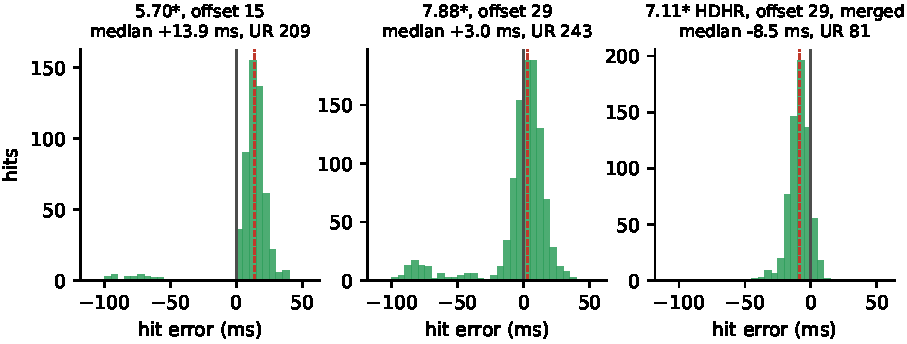
\includegraphics[width=\linewidth]{hit_errors.pdf}
\caption{游戏中记录的按键时间误差（正值为偏晚）。左：校准 offset 之前，按键整体晚约 14\,ms。中：整体居中，
但有一批提前 60--100\,ms 的按键（230 BPM 下恰好提前一拍）。右：合并之后这批早按消失，UR 为 81。}
\label{fig:hits}
\end{figure}

7.88 星谱面的第一局（OD 9.6，300 判定 $\pm22$\,ms）因约 14\,ms 的整体延迟丢掉了大量 300。离线给按键加上 7\,ms 延迟和 15\,ms 随机抖动后，
几乎完全重现了实测结果（73.80\%，646/328/42/17）。判定窗口这么窄时，十几毫秒的时间噪声就足以丢掉大量 300。校准 offset 后提高到 90.09\%。
剩下的 50 和丢掉的 27 个滑条尾都来自重复按键：按游戏规则离线模拟，恰好丢掉 27 个滑条尾。合并按键之后，开启 Hard Rock 的
7.11 星谱面（OD 10，$\pm20$\,ms）打出 96.63\%，没有一个 50，按键时间标准差 8.1\,ms（UR 81），而之前记录的两局 UR 分别为 209 和 243。

\section{讨论}
\paragraph{经验。}
(1) 训练目标的近似可能悄无声息地让方法失效：有限差分惩罚只测到梯度的 $1/\sqrt d$，判别器始终没学会。
(2) 优化设置可能比网络结构更重要：用更高的学习率预训练，让 56.5\% 变成了 96.7\%。
(3) 损失函数决定了模型能表达什么：平方误差无法产生转盘这样的多峰行为，VAE 的转盘损失也有同样缺陷。
(4) 对抗权重过大会以准确率换取真实感。
(5) 对于按键，逐帧预测按住状态使损失对按下时刻不敏感，也容易产生重复按键。
(6) 评估必须与游戏一致：减半的半径、把两个键合并计数的判定都掩盖了真实问题；修正之后，离线预测与实测相差约一个百分点。

\paragraph{局限。}
完整准确率会低估真人，也没有模拟音符锁定和滑条点。``像人''是通过轨迹和统计量（转盘转速、每物件按键次数、UR）来论证的，
没有做感知层面的用户研究。回放延迟在不同局之间会浮动约 10\,ms。合并按键会增加 Miss。游戏内实测只有五局。V3 的数据量仍只有原作者的 79\%。

\paragraph{未来工作。}
让按键模型直接预测按下事件和帧内偏移，对稀少的事件使用 focal 损失或加权损失 \citep{lin2017}，把松开时间绑定到所打物件的结束时刻，
采用非因果 TCN 并以生成的光标为输入，有望在不误删真实按键的前提下消除重复按键。把光标和按键合成一个模型，能让按键依据光标的位置决定。
如果有更多数据，扩散模型 \citep{ho2020, tevet2023} 是光标模型自然的下一步。

\section{伦理声明}
所有游戏内实验都在未登录 osu! 的状态下进行，没有任何成绩被提交到线上排行榜；在线上账号中使用此类回放违反游戏规则，对其他玩家也不公平。
回放程序不包含反检测功能。本文不再分发音乐和谱面文件。osu!3k 数据集依其 MIT 许可使用。

\section*{致谢}
感谢 niooii 的原始项目与模型、GuiBrandt 的 OsuLearn、osu!3k 数据集的作者，以及 tosu 和 osu!lazer 的开发者。
本项目的代码、实验和本文在编写过程中使用了 Claude（Anthropic）作为编程助手。代码见 \url{https://github.com/pekingfather15/osuai}。

\newpage
\renewcommand{\refname}{参考文献}
% Reference list in APA 7th style, shared by paper_en.tex and paper_zh.tex
\begingroup
\setlength{\bibsep}{4pt}
\setlength{\bibhang}{0.5in}
\small
\begin{thebibliography}{99}

\bibitem[{Arjovsky et~al.}(2017)]{arjovsky2017}
Arjovsky, M., Chintala, S., \& Bottou, L. (2017). Wasserstein generative adversarial networks. In D.~Precup \&
Y.~W. Teh (Eds.), \emph{Proceedings of the 34th International Conference on Machine Learning} (Vol.~70,
pp.~214--223). PMLR. \url{https://proceedings.mlr.press/v70/arjovsky17a.html}

\bibitem[{Bai et~al.}(2018)]{bai2018}
Bai, S., Kolter, J.~Z., \& Koltun, V. (2018). \emph{An empirical evaluation of generic convolutional and
recurrent networks for sequence modeling} [Preprint]. arXiv. \url{https://doi.org/10.48550/arXiv.1803.01271}

\bibitem[{Bishop}(2006)]{bishop2006}
Bishop, C.~M. (2006). \emph{Pattern recognition and machine learning}. Springer.

\bibitem[{Bowman et~al.}(2016)]{bowman2016}
Bowman, S.~R., Vilnis, L., Vinyals, O., Dai, A.~M., Jozefowicz, R., \& Bengio, S. (2016). Generating sentences
from a continuous space. In \emph{Proceedings of the 20th SIGNLL Conference on Computational Natural Language
Learning} (pp.~10--21). Association for Computational Linguistics. \url{https://doi.org/10.18653/v1/K16-1002}

\bibitem[{Fitts}(1954)]{fitts1954}
Fitts, P.~M. (1954). The information capacity of the human motor system in controlling the amplitude of
movement. \emph{Journal of Experimental Psychology, 47}(6), 381--391. \url{https://doi.org/10.1037/h0055392}

\bibitem[{Flash \& Hogan}(1985)]{flash1985}
Flash, T., \& Hogan, N. (1985). The coordination of arm movements: An experimentally confirmed mathematical
model. \emph{The Journal of Neuroscience, 5}(7), 1688--1703.
\url{https://doi.org/10.1523/JNEUROSCI.05-07-01688.1985}

\bibitem[{gameswu}(n.d.)]{autosu}
gameswu. (n.d.). \emph{AutOsu} [Computer software]. GitHub. Retrieved October 7, 2026, from
\url{https://github.com/gameswu/AutOsu}

\bibitem[{Gers et~al.}(2000)]{gers2000}
Gers, F.~A., Schmidhuber, J., \& Cummins, F. (2000). Learning to forget: Continual prediction with LSTM.
\emph{Neural Computation, 12}(10), 2451--2471. \url{https://doi.org/10.1162/089976600300015015}

\bibitem[{Goodfellow et~al.}(2014)]{goodfellow2014}
Goodfellow, I., Pouget-Abadie, J., Mirza, M., Xu, B., Warde-Farley, D., Ozair, S., Courville, A., \& Bengio, Y.
(2014). Generative adversarial nets. In \emph{Advances in Neural Information Processing Systems} (Vol.~27).
Curran Associates.

\bibitem[{Graves}(2013)]{graves2013}
Graves, A. (2013). \emph{Generating sequences with recurrent neural networks} [Preprint]. arXiv.
\url{https://doi.org/10.48550/arXiv.1308.0850}

\bibitem[{Gu \& Dao}(2023)]{gu2023}
Gu, A., \& Dao, T. (2023). \emph{Mamba: Linear-time sequence modeling with selective state spaces} [Preprint].
arXiv. \url{https://doi.org/10.48550/arXiv.2312.00752}

\bibitem[{GuiBrandt}(n.d.)]{osulearn}
GuiBrandt. (n.d.). \emph{OsuLearn} [Computer software]. GitHub. Retrieved October 7, 2026, from
\url{https://github.com/GuiBrandt/OsuLearn}

\bibitem[{Gulrajani et~al.}(2017)]{gulrajani2017}
Gulrajani, I., Ahmed, F., Arjovsky, M., Dumoulin, V., \& Courville, A.~C. (2017). Improved training of
Wasserstein GANs. In \emph{Advances in Neural Information Processing Systems} (Vol.~30). Curran Associates.

\bibitem[{Ho et~al.}(2020)]{ho2020}
Ho, J., Jain, A., \& Abbeel, P. (2020). Denoising diffusion probabilistic models. In \emph{Advances in Neural
Information Processing Systems} (Vol.~33, pp.~6840--6851). Curran Associates.

\bibitem[{Hochreiter \& Schmidhuber}(1997)]{hochreiter1997}
Hochreiter, S., \& Schmidhuber, J. (1997). Long short-term memory. \emph{Neural Computation, 9}(8), 1735--1780.
\url{https://doi.org/10.1162/neco.1997.9.8.1735}

\bibitem[{Hussein et~al.}(2017)]{hussein2017}
Hussein, A., Gaber, M.~M., Elyan, E., \& Jayne, C. (2017). Imitation learning: A survey of learning methods.
\emph{ACM Computing Surveys, 50}(2), Article 21. \url{https://doi.org/10.1145/3054912}

\bibitem[{ilymeow}(n.d.)]{osu3k}
ilymeow. (n.d.). \emph{osu!3k} [Data set]. Kaggle. Retrieved October 7, 2026, from
\url{https://www.kaggle.com/datasets/ilymeow/osu3k}

\bibitem[{Isola et~al.}(2017)]{isola2017}
Isola, P., Zhu, J.-Y., Zhou, T., \& Efros, A.~A. (2017). Image-to-image translation with conditional adversarial
networks. In \emph{Proceedings of the IEEE Conference on Computer Vision and Pattern Recognition}
(pp.~1125--1134). IEEE. \url{https://doi.org/10.1109/CVPR.2017.632}

\bibitem[{Kingma \& Ba}(2015)]{kingma2015}
Kingma, D.~P., \& Ba, J. (2015). Adam: A method for stochastic optimization. In \emph{3rd International
Conference on Learning Representations}. \url{https://doi.org/10.48550/arXiv.1412.6980}

\bibitem[{Kingma \& Welling}(2014)]{kingma2014vae}
Kingma, D.~P., \& Welling, M. (2014). Auto-encoding variational Bayes. In \emph{2nd International Conference on
Learning Representations}. \url{https://doi.org/10.48550/arXiv.1312.6114}

\bibitem[{Lin et~al.}(2017)]{lin2017}
Lin, T.-Y., Goyal, P., Girshick, R., He, K., \& Doll\'ar, P. (2017). Focal loss for dense object detection. In
\emph{Proceedings of the IEEE International Conference on Computer Vision} (pp.~2980--2988). IEEE.
\url{https://doi.org/10.1109/ICCV.2017.324}

\bibitem[{minetoblend}(n.d.)]{osucad}
minetoblend. (n.d.). \emph{osucad-cursor-predict} [Computer software]. GitHub. Retrieved October 7, 2026, from
\url{https://github.com/minetoblend/osucad-cursor-predict}

\bibitem[{Mirza \& Osindero}(2014)]{mirza2014}
Mirza, M., \& Osindero, S. (2014). \emph{Conditional generative adversarial nets} [Preprint]. arXiv.
\url{https://doi.org/10.48550/arXiv.1411.1784}

\bibitem[{Neubeck \& Van~Gool}(2006)]{neubeck2006}
Neubeck, A., \& Van Gool, L. (2006). Efficient non-maximum suppression. In \emph{18th International Conference
on Pattern Recognition} (Vol.~3, pp.~850--855). IEEE. \url{https://doi.org/10.1109/ICPR.2006.479}

\bibitem[{Neuro-sama}(n.d.)]{neurosama}
Neuro-sama. (n.d.). In \emph{Wikipedia}. Retrieved October 7, 2026, from
\url{https://en.wikipedia.org/wiki/Neuro-sama}

\bibitem[{niooii}(2026)]{niooii}
niooii. (2026). \emph{osu} [Computer software]. GitHub. \url{https://github.com/niooii/osu}

\bibitem[{Plumerault et~al.}(2020)]{plumerault2020}
Plumerault, A., Le Borgne, H., \& Hudelot, C. (2020). \emph{AVAE: Adversarial variational auto encoder}
[Preprint]. arXiv. \url{https://doi.org/10.48550/arXiv.2012.11551}

\bibitem[{Pomerleau}(1989)]{pomerleau1989}
Pomerleau, D.~A. (1989). ALVINN: An autonomous land vehicle in a neural network. In D.~S. Touretzky (Ed.),
\emph{Advances in Neural Information Processing Systems} (Vol.~1, pp.~305--313). Morgan Kaufmann.

\bibitem[{ppy}(n.d.-a)]{lazer}
ppy. (n.d.-a). \emph{osu!} [Computer software]. GitHub. Retrieved October 7, 2026, from
\url{https://github.com/ppy/osu}

\bibitem[{ppy}(n.d.-b)]{wikics}
ppy. (n.d.-b). Circle size. In \emph{osu! wiki}. Retrieved October 7, 2026, from
\url{https://osu.ppy.sh/wiki/Beatmap/Circle_size}

\bibitem[{ppy}(n.d.-c)]{wikiod}
ppy. (n.d.-c). Overall difficulty. In \emph{osu! wiki}. Retrieved October 7, 2026, from
\url{https://osu.ppy.sh/wiki/Beatmap/Overall_difficulty}

\bibitem[{Rezende et~al.}(2014)]{rezende2014}
Rezende, D.~J., Mohamed, S., \& Wierstra, D. (2014). Stochastic backpropagation and approximate inference in deep
generative models. In \emph{Proceedings of the 31st International Conference on Machine Learning} (Vol.~32,
pp.~1278--1286). PMLR.

\bibitem[{Ross et~al.}(2011)]{ross2011}
Ross, S., Gordon, G., \& Bagnell, D. (2011). A reduction of imitation learning and structured prediction to
no-regret online learning. In \emph{Proceedings of the Fourteenth International Conference on Artificial
Intelligence and Statistics} (Vol.~15, pp.~627--635). PMLR.

\bibitem[{Tevet et~al.}(2023)]{tevet2023}
Tevet, G., Raab, S., Gordon, B., Shafir, Y., Cohen-Or, D., \& Bermano, A.~H. (2023). Human motion diffusion
model. In \emph{The Eleventh International Conference on Learning Representations}.
\url{https://doi.org/10.48550/arXiv.2209.14916}

\bibitem[{tosu}(n.d.)]{tosu}
tosu. (n.d.). \emph{tosu} [Computer software]. GitHub. Retrieved October 7, 2026, from
\url{https://github.com/tosuapp/tosu}

\bibitem[{van~den Oord et~al.}(2016)]{oord2016}
van den Oord, A., Dieleman, S., Zen, H., Simonyan, K., Vinyals, O., Graves, A., Kalchbrenner, N., Senior, A.,
\& Kavukcuoglu, K. (2016). \emph{WaveNet: A generative model for raw audio} [Preprint]. arXiv.
\url{https://doi.org/10.48550/arXiv.1609.03499}

\bibitem[{Vaswani et~al.}(2017)]{vaswani2017}
Vaswani, A., Shazeer, N., Parmar, N., Uszkoreit, J., Jones, L., Gomez, A.~N., Kaiser, \L., \& Polosukhin, I.
(2017). Attention is all you need. In \emph{Advances in Neural Information Processing Systems} (Vol.~30).
Curran Associates.

\bibitem[{Yu \& Koltun}(2016)]{yu2016}
Yu, F., \& Koltun, V. (2016). Multi-scale context aggregation by dilated convolutions. In \emph{4th
International Conference on Learning Representations}. \url{https://doi.org/10.48550/arXiv.1511.07122}

\end{thebibliography}
\endgroup


\end{document}
